% Chapter 4

\section{Architecture}
\label{sec:Architecture}
% UML diagrams, source code, SSE, ERD diagrams
The software was built following the Ruby on Rails conventions, namely the MVC (Model-View-Controller)
pattern. A more accurate name would be Model-Controller-View, if is to show the
depth in the software stack of each component. The Model is the one interacting with the
database (managed by MySQL, or in our case PostgreSQL). The controllers are sending and
receiving data, filtering it, send redirect headers, and rendering templates. The Views
are the components that the user gets to see them, they are templates that are rendered
on the browsers, and interpolate data made available by the controller.
The \textit{Course} model shown in Listing~\ref{course} is the most important in the system.
It doesn't do much, it defines a relation to the \textit{User} model and has some validations
that prevent users from abusing the system.
\begin{lstlisting}[language=Ruby, caption={Course Model}, label=course]
# @author Dumitru Ursu
# Model for courses
class Course < ActiveRecord::Base
  belongs_to :user
  has_attached_file :slides
  validates_attachment_content_type :slides, content_type: [
    'application/vnd.oasis.opendocument.presentation', 'application/pdf',
    'text/html']
end
\end{lstlisting}
Switching from Rails 3.1 to the 4-th version, made the model even more compact, by implementing
\textit{ActiveModel::Model}. The new version also allows create a new class and be able to update its attributes through a form,
like an \textit{ActiveModel} object, but not persist it to the database.
Previously the attributes were listed within the model,but now they are only present in the
\textit{CourseController} filters and migrations. In the class diagram of the system the attributes
and methods are also shown, in Figure~\ref{fig:Class Diagram}.
\begin{figure}[ht!]
    \centering
    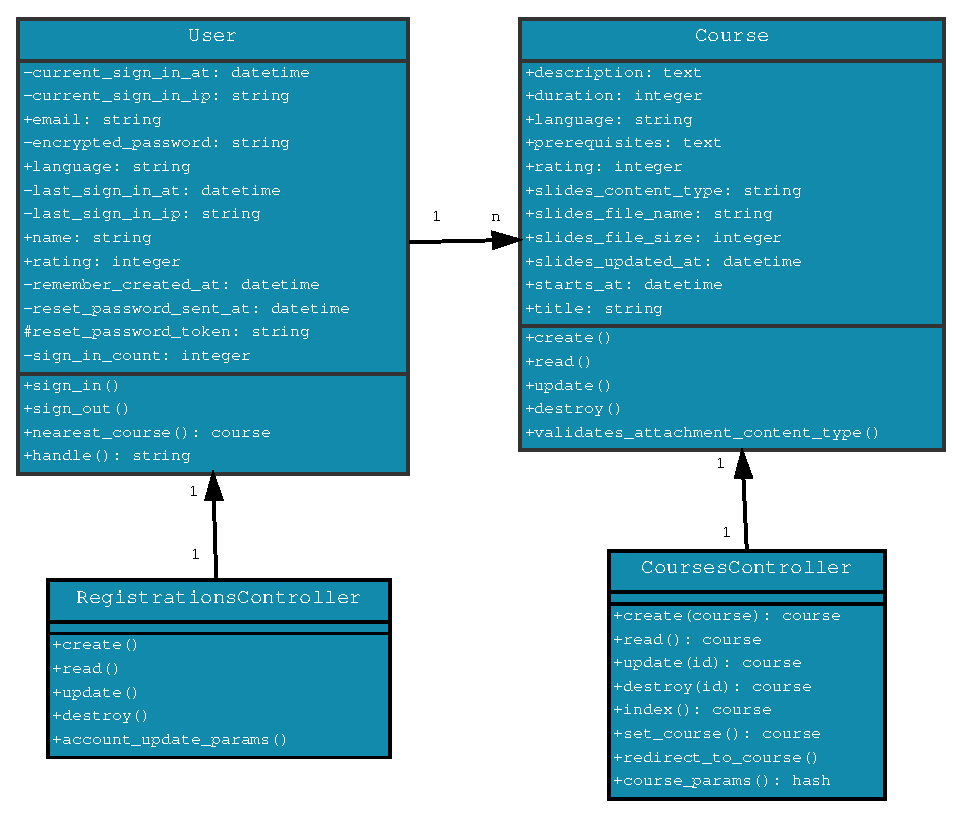
\includegraphics{class}
    \caption{Class diagram of system components}
    \label{fig:Class Diagram}
\end{figure}

\subsection{Rails migrations}
Rails provides a mechanism to modify the database schema, and also keeping all the
data in place, if one is careful enough. Migrations use a Ruby DSL so that one
doesn't have to write SQL by hand, allowing the schema and changes to be database
independent. For example, in Listing~\ref{slidesmig} several columns are added
with the \textit{add\_attachment} command. It may not be seem so, but this DSL predicate
is provided by \textit{PaperClip}, a library that ease easy file attachment library for
Active Record.
\textit{PaperClip} \textit{add\_attachment} wraps 4 attributes:
\begin{enumerate}
    \item[--] $\langle attachment\rangle$\_file\_name;
    \item[--] $\langle attachment\rangle$\_file\_size;
    \item[--] $\langle attachment\rangle$\_content\_type;
    \item[--] $\langle attachment\rangle$\_updated\_at.
\end{enumerate}
The \textit{Paperclip} attributes are all prefixed with that attachment's name, in this case
the HTML file that is being uploaded as a presentation.
This allows to have multiple attachments per model, and give them a friendly front end.
The intent behind it was to keep setup as easy as possible and to treat files as much like other attributes as possible.
The next features that will be implemented with \textit{PaperClip} is avatars for users.
\begin{lstlisting}[language=Ruby, caption={Slides migration}, label=slidesmig]
class AddSlidesColumnToCourses < ActiveRecord::Migration
  def self.up
    add_attachment :courses, :slides
  end

  def self.down
    remove_attachment :courses, :slides
  end
end
\end{lstlisting}
The \textit{self.down} event is triggered when the database is reverted to a previous state,
past the point when this migration was created. All migrations are timestamped
to keep track of how the database was created, and in what order should the database
be rolled back  as shown in this listing \ref{ls_migrations}. \begin{lstlisting}[language=Bash, caption={The migration directory}, label=ls_migrations]
20130923040646_devise_create_users.rb
20131005225555_create_courses.rb
20131031112018_add_rating_to_courses.rb
20131031112055_add_rating_to_users.rb
20140210142725_add_name_to_users.rb
20140210174537_add_duration_to_courses.rb
20140213021746_add_language_to_users.rb
20140228161213_add_slides_column_to_courses.rb
\end{lstlisting}
These are not created by hand, (although one could create the files like that),
instead most of the time Rails developers rely on a migrations generator. The
names of the migrations are self-explanatory.

\subsection{Client-side architecture}
As mentioned at the beginning of the Chapter~\ref{sec:Architecture}, the interface is generated from the views file.
The views in their turn interact with the controller. It is possible to access the models
directly form the views, but this is bad practice, as the user interfaces gets mixed with
business logic, and becomes very hard to change. This requests paths and interaction between
the mentioned Rails components is shown in Figure~\ref{rails_mvc}.
\begin{figure}[ht!]
\centering
\includegraphics[height=10cm]{rails_mvc}
\caption{Rails components interaction}
\label{rails_mvc}
\end{figure}

The views use a special templating language: by default is .erb, which stands for
embedded ruby, and is basically HTML with a new tag for embedding ruby scripts,
but in Discite it was replaced with Haml (HTML abstraction markup language). Haml
looks and feels a lot like Python code, in the sense that is very concise and it
relies on indentation for scoping, instead of braces or tags. This can be seen in
Listing~\ref{courseform}, where the form for creating, editing and updating courses
is described. This might seem like a long and intricate form, but it is
rendered in over 250 lines of pure HTML, and is rendered in the browser window as shown
in Figure~\ref{fig:course_creation}.
\begin{lstlisting}[language=Python, caption={Course creation template}, label=courseform]
= form_for @course, :html => { :multipart => true } do |f|
  - if @course.errors.any?
    #error_explanation
      %h2= "#{pluralize(@course.errors.count, "error")} prohibited this course from being saved:"
      %ul
        - @course.errors.full_messages.each do |msg|
          %li= msg
  .row
    .columns.large-8.small-6
      = f.label :title
      = f.text_field :title
    .columns.large-4.small-6
      = f.label :language
      = f.select :language, LanguageList::COMMON_LANGUAGES.map{ |language| [language.name, language.iso_639_1] }
  = f.label :description
  = f.text_area :description, rows: 8
  = f.label :prerequisites
  = f.text_area :prerequisites, rows: 6
  = f.label 'Slides'
  = f.file_field :slides
  .row
    .columns.large-10
      = f.label 'Starting Date'
      = datetime_select :course, :starts_at, {time_separator: '', datetime_separator: '',
        prompt: true}, {class: 'large-2 columns end'}
    .columns.large-2
      = f.label 'Duration (hours)'
      = f.text_field :duration, type: 'number'
  = f.submit 'Save', class: 'button'
\end{lstlisting}

\subsection{Assets management}
A subsystem of Rails takes care of minifying and compressing CSS and JavaScript
files. This system is called the asset pipeline.
Beside the aforementioned features, the pipleline also has the ability to write
these assets in other languages and pre-processors such as CoffeeScript, Sass
and ERB and the templating language of choice from this project, Haml.
The asset pipeline is no longer a core feature of Rails 4, it has been extracted
out of the framework into the \textit{sprockets-rails} gem, and in fact, most of it's job
is done by Bower in this project.
Bower is a package manager for the web, built by Twitter. It offers a generic
solution to the problem of front-end package management, while exposing the
package dependency model via an API that can be consumed by a more opinionated
build stack, in this case the Rails default asset pipeline. There are no system
wide dependencies, no dependencies are shared between different apps, and the
dependency tree is flat.

Like some other similar projects, Bower runs over Git, and is package-agnostic.
It was the only one that was reliable enough, and provide enough packages for this
project, after several failed attempts. A packaged component can be made up of any type of asset, and
use any type of transport. In this project case, we use git and SSH protocol to get
the data in the project, then commit it, and then is pushed to the server via SSH.
One way of optimizing this process would be to concatenate the server on the local
machine, and then send them to the remote server, but this has yet to be investigated.

As more CSS frameworks, the JavaScript librariels began to clump up
the project, it became clear that the standard pipeline could no longer handle the management of the assets.
At this time, in fact sprockets still concatenates, minifies and compresses assets, but the way they are
installed in the project is different, as seen in Figure \ref{fig:deployment}
\begin{figure}[ht!]
    \centering
    \includegraphics[height=8cm,keepaspectratio]{deployment}
    \caption{Deployment diagram}
    \label{fig:deployment}
\end{figure}

Some of the trials and errors with asset management ranged from purely using the
pipepline (which has been inadequate for this project), to using git submodules,
manually installing JS files, jammit, and systems that gemify automatically
libraries from git repositories.
In this case, accommodating Rails and Bower was quite a easy and scalable way to go.
\begin{lstlisting}[language=JavaScript, caption={Bower.json file}, label=bower]
version": "0.0.1",
  "authors": [
    "Dumitru Ursu <dima@ceata.org>"
  ],
  "description": "\"A peer to peer teaching network\"",
  "main": "bower.json",
  "moduleType": [
    "globals"
  ],
  "license": "MIT",
  "homepage": "discite.info",
  "private": true,
  "ignore": [
    "**/.*",
    "node_modules",
    "bower_components",
    "vendor/assets/components",
    "test",
    "tests"
  ],
  "dependencies": {
    "deck.js": "~1.1.0",
    "deck.annotate.js": "~0.0.0",
    "sisyphus": "1.1.103",
    "foundation": "5.2.2",
    "jquery": "2.1.0",
  }
}
\end{lstlisting}

Assets installed this way need to be loaded into sprokets, so minification, concatenation and compression
will happen automatically, and this is done in Listing~\ref{enable_bower}.
\begin{lstlisting}[language=Ruby, caption={Plugging Bower into the assets pipeline}, label=enable_bower]
module Discite
  class Application < Rails::Application
    # Application configuration should go into files in config/initializers
    # -- all .rb files in that directory are automatically loaded.
    config.i18n.enforce_available_locales = true
    config.i18n.load_path += Dir[Rails.root.join('config', 'locales', '*.{rb,yml}').to_s]
    config.i18n.default_locale = :en
    config.assets.paths << Rails.root.join('app', 'assets', 'fonts', 'vendor', 'components')
  end
end
\end{lstlisting}

\subsection{Storage}
There are 2 main type of storage used by the Discite platform: \textit{localStorage} and  \textit{PosgreSQL}
The first is used by a library called \textit{Sysiphus}, that saves HTML forms data to
\textit{localStorage} to restore them after browser crashes, tabs closings and other
disasters. This way, our users will not have to refill the form for course creation,
if anything bad happens and as the form has become quite big, this was a very welcomed improvement.
The course creation process is shown in Figure~\ref{fig:course_management}.
\begin{figure}[ht!]
    \centering
    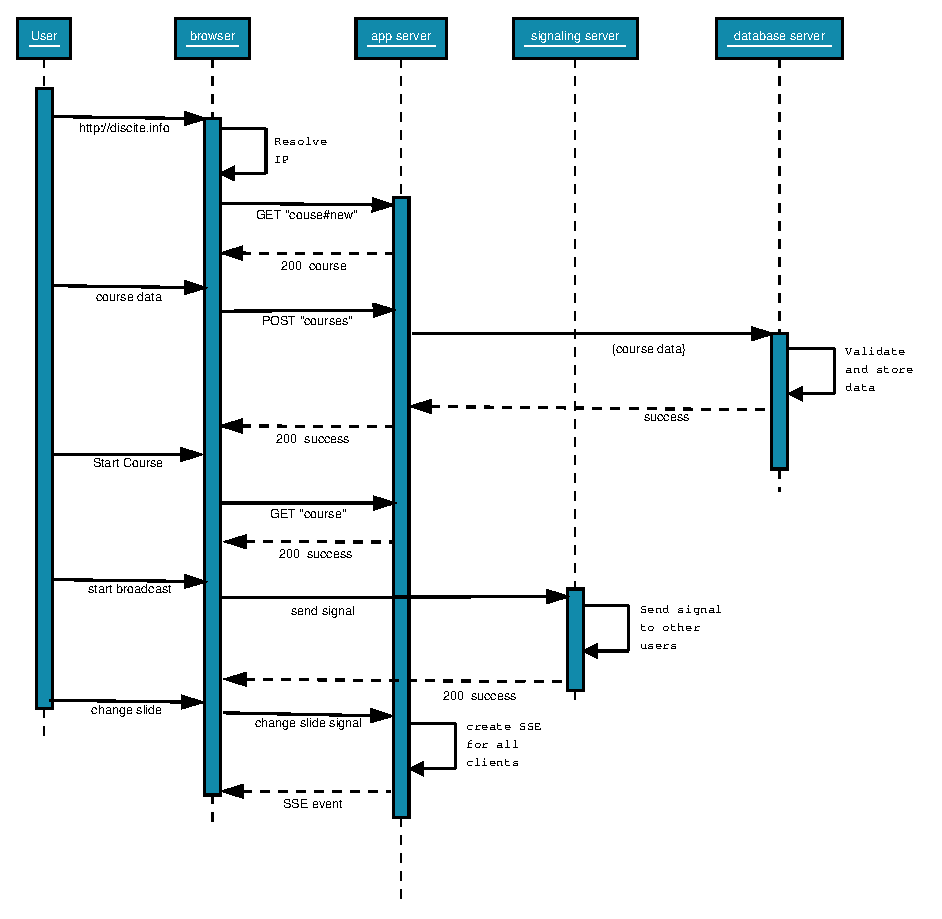
\includegraphics[height=20cm,width=\textwidth, keepaspectratio]{s_course_management}
    \caption{Sequence diagram for course management}
    \label{fig:course_management}
\end{figure}

\textit{localStorage} is a  way for web pages to store named key/value pairs locally, within
the client web browser. Like cookies, this data persists even after you navigate
away from the web site, close your browser tab, exit your browser. Unlike
cookies, this data is never transmitted to the remote web server
(unless you specifically do that). Unlike all previous
attempts at providing persistent local storage, it is implemented natively in
web browsers, so it is available even when third-party browser plugins are not.

The second type of storage is on the server side, where PostgreSQL is used,
often simply "Postgres",that is an object-relational database management
system (ORDBMS) with an emphasis on extensibility and standards-compliance. As a
database server, its primary function is to store data, securely and supporting
best practices, and retrieve it later, as requested by other software
applications, be it those on the same computer or those running on another
computer across a network (including the Internet). It can handle workloads
ranging from small single-machine applications to large Internet-facing
applications with many concurrent users. Recent versions also provide
replication of the database itself for security and scalability.

In fact, ActiveRecord provides some nice abstractions around the whole SQL concept,
and Posgres can be easily exchanged for another RDBMS vendor that has support
with ActiveRecord, such as MySQl, Oracle, or MSSQL.
ActiveRecord allows programmers to programmatically define a schema in a
portable DSL. This means you can define tables, indexes, etc. without using SQL
directly, so your applications can more easily support multiple databases, as shown in Listing~\ref{arschema}.
\begin{lstlisting}[language=Ruby, caption={ActiveRecord Schema definition}, label=arschema]
ActiveRecord::Schema.define do
  create_table :users do |t|
    t.string :name, null: false
  end

  add_index :users, :name

  create_table :posts do |t|
    t.integer :user_id, null: false
    t.string :name
    t.text :body
    t.boolean :private, default: false
  end

  add_index :posts, :author_id
end
\end{lstlisting}

This comes at a price though, as more advanced features that PostgreSQL supports are
being left out of the abstraction, like HStore.
HStore functions much like serializing hashes, except that data can be queried
much faster since HStore is a native data type. It is not  supported natively in
Rails 4, but until then we’ll need to use the \textit{activerecord-postgres-hstore} gem,
and this would make our code depend on a specific RDBMS. When this is not an
issue, higher performance can be gained from this move, as \textit{Course}
and \textit{User} models can be stored directly as hashes, without going though
several cycles of serialization/deserialization.
This functionality requires a recent version of PostgreSQL that supports the HStore
extension.The extension can be enabled by running the migration from Listing~\ref{hstore_enable}.
\begin{lstlisting}[language=Ruby, caption={Enable HStore Postgres extension}, label=hstore_enable]
class SetupHstore < ActiveRecord::Migration
  def self.up
    execute "CREATE EXTENSION hstore"
  end

  def self.down
    execute "DROP EXTENSION hstore"
  end
end
\end{lstlisting}

After this is done, it is possible to create a column with a type of HStore, here
we are giving our User model a column called data with HStore type.

\begin{lstlisting}[language=Ruby, caption={Hstore for User model}, label=hstore_course]
class CreateUser < ActiveRecord::Migration
  def change
    create_table :user do |t|
      t.string  :name
      t.hstore  :data
      t.timestamps
    end
  end
end
\end{lstlisting}
Users can then be created by following the user registration process, presented in the Figure~\ref{fig:user_creation},
or by creating them manually, at Rails console, like in Listing~\ref{hstore_user_creation}.
The second process could be of use if a university or school is doing mass-enrollment of students,
and already has their data, or the registration page is taken down, to stop unknown people from registering
on the website, basically making it a private site.
\begin{figure}[ht!]
    \centering
    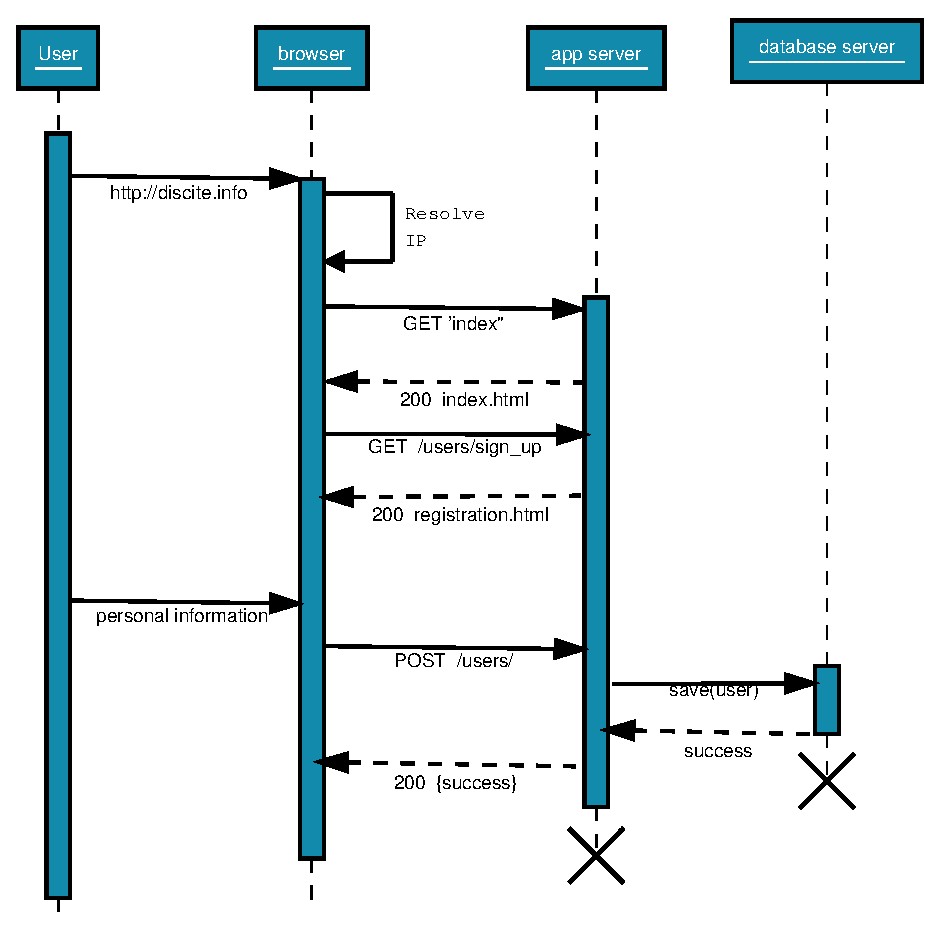
\includegraphics[height=13cm]{s_user_creation}
    \caption{Sequence diagram for user creation}
    \label{fig:user_creation}
\end{figure}

\begin{lstlisting}[language=Ruby, caption={Creating a new User}, label=hstore_user_creation]
User.create(:name => "George Popescu", :data => {'email' => 'g.popescu@gmail.com', 'age' => 18, 'group' => '11B'})
User.last.data['age']  # => 18
\end{lstlisting}


This kind of persistent storage is used for user data and courses. The hierarchical filesystem is used to
store the presentation files. Storing them in the RDBMS is considered, but was not
implemented because there were no reasons for it yet, but scalability and integrity of
data might become a concern for the slides files.
Moving files in the RDMS brings some advantages, like the following:
\begin{enumerate}
    \item[--] When storing files in the database there is a guarantee that the data
        is consistent. The foreign keys will enforce referential integrity. It
        is relatively hard to execute transactional operations on both the file
        system and the database at the same time. This is the most important
        reason why the switch should be made;
    \item[--] When all the user generated data is in the database it is easier
        to maintain. In order to backup the data we will only backup the database.
        While it is not that hard to backup some files it is still a
        concern and is spreading the effort and the area where errors can occur.
        What is more, if at some point there is a change in
        the application that requires some update to the existing data like
        changing the file names to match some convention or adding a watermark
        to the slides it is easier to manipulate data using SQL than writing a
        custom tool to crawl through files and directories, and having more services
        to maintain;
    \item[--] One can store file related metadata like file size, image
        dimensions, filenames  and make queries over it:  if this data is
        "attached" to the file and it is easier to preserve data integrity.
\end{enumerate}

\subsection{Future Architetural Improvements}
One major improvement would be implementation of a management dashboard for the teacher, to allow better course
management. The software is does not currently provide means to block abusive students, for example. A set of
features that are planned at latter versions are:
\begin{enumerate}
    \item[--] System for sorting, and approving students;
    \item[--] A enrollment key system;
    \item[--] PDF support for presentations;
    \item[--] Ratings for students and courses;
    \item[--] Featured courses/teachers;
    \item[--] HTML editor for presentations, based on Scribe from Guardian.
\end{enumerate}

The search system that is based on \textit{FortyFacets}, a library for
building explorative search interfaces, implemented as shown in Listing~\ref{search} is
not working reliably, and doesn't support users/teacher searches for the moment.
\begin{lstlisting}[language=Ruby, caption={Course Search controller}, label=search]
class CourseSearch < FortyFacets::FacetSearch
    model 'Course'
    text :title
    range :duration, name: 'Duration'
    facet :language, name: 'Language'
    facet :starts_at, name: 'Starting date', order: :starts_at
    facet :rating, name: 'Rating', order: :rating
  end
\end{lstlisting}

The User search shown in Listing~\ref{user_search} poses privacy concerns, and can't have a full implementation at the moment.
Most of the fieds are stripped away (email, age) due to these concerns. The best solution found
is to have Privacy Preferences inside the profile page, but this requires a highly elaborate User model,
and lots of tweaking to the system, so it won't crash if the needed data is not made availble.
\begin{lstlisting}[language=Ruby, caption={User search controller}, label=user_search]

  class UserSearch < FortyFacets::FacetSearch
    model 'User'
    text :name
    #add rating to to user search
  end

  def courses
    @search = CourseSearch.new(params) # this initializes your search object from the request params
    @course = @search.result.paginate(page: params[:page], per_page: 5) # optionally paginate through your results
  end

  def users
    @search = UserSearch.new(params)
    @user = @search.result.paginamte(page: params[:page], per_page: 5)
  end
end
\end{lstlisting}

The biggest leap forward will be achieved if the course page will be rewritten:
a better choice for doing the signaling would have been WebSockets, and
Nodejs with socket.io as is shown in benchmarks to support la larger number of users
that ActiveController::Live is capable of for the moment.
The current implementation is quite simple, as shown in listing \ref{syncronizer}

\begin{lstlisting}[language=Ruby, caption={ActionController::Live syncronizer}, label=syncronizer]
require 'streamer/sse'

class SlidesController < ApplicationController
  include ActionController::Live

  def index
      # SSE expects the `text/event-stream` content type
    response.headers['Content-Type'] = 'text/event-stream'

    sse = Streamer::SSE.new(response.stream)

    begin
      sse.write(params.permit(:slide), event: 'slide_change')
    rescue IOError
      # When the client disconnects, we'll get an IOError on write
    ensure
      sse.close
    end
    render nothing: true
  end
end
\end{lstlisting}

\subsubsection{Service Oriented Architecture}
Because of the possible rewrite of the application core feature, the course page,
an alternative architecture is considered. The current monolithic architecture is
hard to change, and hard to adapt to changes. On the bright side, the application is easy
to deploy, having only one component to take care of, and this is done so by design.

A service-oriented architecture is essentially a collection of services. These
services communicate with each other via a certain protocol. The communication can involve either
simple data passing or it could involve two or more services coordinating some
activity. Some means of connecting services to each other is needed, and for this
a REST API might be considered, which is a popular way to consume and create services,
as it's easy to create, read, update or delete information on a server using simple HTTP calls.

\clearpage

